\documentclass{beamer}
\usepackage{beamerthemeshadow}
\usetheme{Warsaw}
\usepackage{graphicx}
\usepackage{caption,subcaption}
%\usepackage[showframe]{geometry}
\usepackage{color}
\usepackage[utf8]{inputenc}
\usepackage{hyperref}
\usepackage[flushleft]{threeparttable}
\usepackage[T2A]{fontenc}
\usepackage[english,serbian]{babel}
\definecolor{beamer@darkerblue}{rgb}{0.1.5,0.2,0.35}
\definecolor{beamer@ibmblue}{rgb}{0.3,0.42,0.7}
\setbeamercolor{structure}{fg=beamer@ibmblue}
\setbeamercolor{section in head/foot}{bg=beamer@darkerblue}

\def\d{{\fontencoding{T1}\selectfont\dj}}
\def\D{{\fontencoding{T1}\selectfont\DJ}}

\title[]{Kompanija IBM}
\subtitle{-- Seminarski rad --}
\author[]{Staša Đorđević\and
Jovana Medenica\\\and  
Marko Veljović\and
Matija Radulović}
\institute[]{Matematički fakultet\\Univerzitet u Beogradu}
\date{
    \footnotesize{Beograd, 2022.}	
}

\begin{document}

\begin{frame}
	\thispagestyle{empty}
	\titlepage
\end{frame}

\begin{frame}[fragile]\frametitle{Literatura}
	\begin{itemize}
		\item Zasnovano na:\\
		Chronological History of IBM
		(\url{https://www.ibm.com/ibm/history/history/history_intro.html})
	\end{itemize}
\end{frame}

\begin{frame}
	\frametitle{Pregled} % Table of contents slide, comment this block out to remove it
	\tableofcontents[hidesubsections] 
\end{frame}

\section{Rana istorija kompanije}

\begin{frame}[fragile]\frametitle{Nastanak kompanije IBM}
	\begin{itemize}	
		\item Koreni se naziru krajem 19. veka
		\item Postojale su četiri male kompanije koje su se kasnije spojile u IBM
		\item Herman Holerit - popis stanovništva 1890.
		\item Kompanija CTR kao preteča IBM-a
		\item Tomas J. Votson - THINK
		\item Od 1924. godine zvaničan naziv je IBM (eng.~{\em International Business Machines})
		\end{itemize}
\end{frame}

\section{IBM sredinom proslog veka}

\begin{frame}[fragile]\frametitle{IBM sredinom prošlog veka}
	\begin{itemize}	
		\item Uticaj Velike ekonomske krize na kompaniju
		\item Ugovor sa američkom vladom - ključan potez za prolazak kroz težak period
		\item Beneficije za zaposlene za vreme krize
            \item Drugi svetski rat, stanje kompanije za vreme sukoba svetskih razmera
            \item Privremeno prilagođavanje proizvodnje novom tržištu
            \item Smrt Votsona Seniora, dolazak mlađe generacije
            \item Zlatno doba
	\end{itemize}
\end{frame}


\section{Najbitniji izumi}
\begin{frame}[fragile]\frametitle{Najbitniji izumi}
\begin{columns}
\column{0.84\linewidth}
	\begin{itemize}	
	\setlength{\itemindent}{3em}
		\item IBM 603, 701
		\item IBM 650, 1401	
		\item Porodica računara Sistem/360
		\item IBM 5100, PC
		\item Magnetna traka, hard disk, DRAM
		\item Relacione baze, SQL
		\item Nobelove nagrade, standardi i protokoli
		\end{itemize}
		\column{0.38\linewidth}
		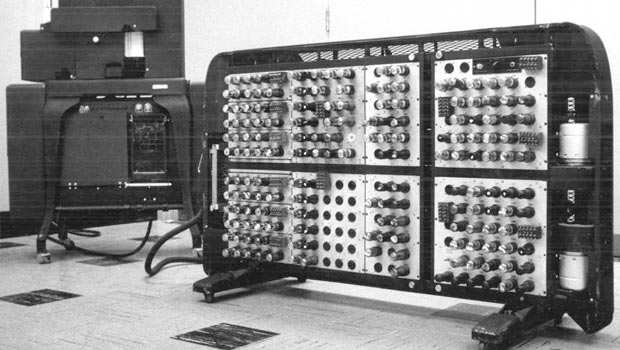
\includegraphics[width=0.77\linewidth]{ibm603.jpg}
  %\caption{IBM 603}
  \label{fig:1}
  %\medskip
  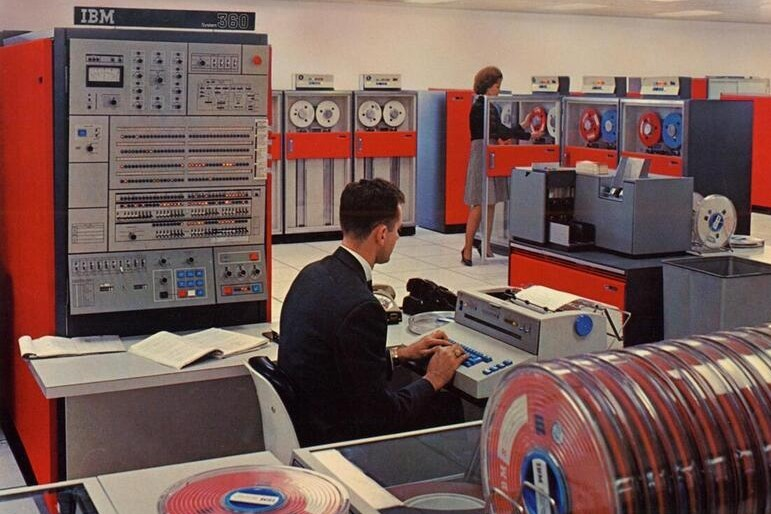
\includegraphics[width=0.77\linewidth]{sys360.jpg}
  %\caption{Sistem 360}
  \label{fig:2}
  %\medskip
  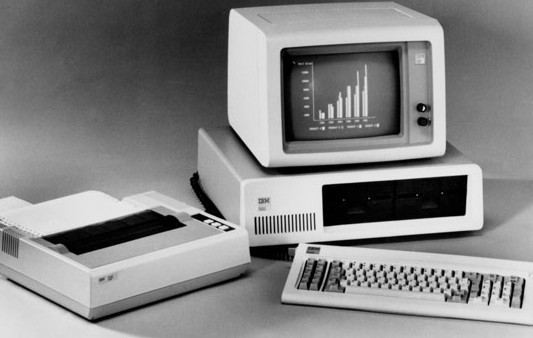
\includegraphics[width=0.77\linewidth]{ibmpc2.jpg}
  %\caption{IBM PC}
  \label{fig:3}
\end{columns}
\end{frame}
%\begin{frame}[fragile]\frametitle{Najbitniji izumi}

%\end{frame}
\section{Razvoj ličnih računara i pad IBM-a}
\begin{frame}[fragile]\frametitle{Razvoj ličnih računara i pad IBM-a}
	\begin{itemize}
	\item Propust u razvoju minikompjutera, nije ispratila tržište
	\item Povratak u doba ličnih računara
	\begin{itemize}
	\item IBM 5100
	\item IBM PC
	\item IBM PC AT
	\end{itemize}
	\item Pravi niz pogrešnih odluka koje je skupo koštaju
	\item Proizvodnju operativnog sistema prepušta Majkrosoftu(eng.~{\em Microsoft})
	\item Proizvodnju mikroprocesora prepušta Intelu
	\item Da bi se povratila menja fokus sa hardvera na razvoj softvera
	\end{itemize}
\end{frame}



\section{IBM danas}

\begin{frame}[fragile]\frametitle{IBM danas}
	\begin{itemize}	
		\item IBM godinama dominantna kompanija
		\item Prodaja PC kompaniji Lenovo 
		\item Trenutno se bave cloud servisima i veštačkom inteligencijom
            \item Projekat Watson
            \item IBM se 2021. godine deli na dva dela
            \begin{itemize}
	       \item Managed Infrastructure Services
	       \item Hibridna cloud platforma i veštačka inteligencija
	    \end{itemize}
            
	\end{itemize}
\end{frame}

\section{Zakljucak}

\begin{frame}[fragile]\frametitle{Zaključak}
	\begin{itemize}	
	\item Kompanija IBM je doživela velike uspone i padove od osnivanja pa do sada.
        \item Pitanje je, da li se može vratiti među vodeće u svetu računarstva?
        \item Uprkos svemu tome, ostavila je dubok trag u istoriji i razvoju tehnologije kakvu danas znamo.
	\end{itemize}
\end{frame}


\end{document}
